\documentclass{beamer}

\usepackage{graphicx}
\usepackage[utf8]{inputenc}
\usepackage[T1]{fontenc}
\usepackage{lmodern}
\usepackage{euler}
\usepackage{enumitem}
\usepackage{outlines}
\usepackage{color}
\usepackage{xcolor}
\usepackage{soul}
\usetheme{AnnArbor}
\usepackage{graphicx}
\usepackage{enumitem}
\usepackage{tikz}
\usepackage{comment}
\def\checkmark{\tikz\fill[scale=0.4](0,.35) -- (.25,0) -- (1,.7) -- (.25,.15) -- cycle;}
\title{About the Google App Engine}
\author{ Tobias Reincke}

\begin{document}
	%	\author{Tobias Reincke}
	
	\title{Presentation about Platform as a service}
	%\subtitle{}
	%\logo{}
	%\institute{}
	%\date{}
	%\subject{Google App Engine}
	\setbeamercovered{transparent}
	%\setbeamertemplate{navigation symbols}{}
\begin{frame}[plain]
    \maketitle
\end{frame}

\begin{frame}{Introduction / What is this Presentation as a Service? }
	\begin{enumerate}[label=]
		\item service allowing development, management and running without building infrastructure
		\item Typical for app development
		\item shortened to PaaS
		
	
		\begin{itemize}
				\item \footnotesize{ $\rightarrow$ Focus on Google App Engine} 
		\end{itemize}
		\item Is being delivered in 3 ways (definitions): 
	\end{enumerate}
\end{frame}
\begin{frame}{Development \& Uses}
    \centering
	--\textbf{ Public} --
	
	\begin{itemize}
	 \item consumer controlls deployment
	 \item minimal configurations
	 \item is provided:
	 
	 \begin{enumerate}[label= \Alph*]
	 	\centering
	 		 \item server and networks 
	 	\item storage 
	 	\item operating system 
	 	\item middleware (like Java Runtime, .NET)
	 	\item database services
	 	\item other services
	 				\item uses virtual machines host and scale services
	 \end{enumerate}

	\end{itemize}
\end{frame}
\begin{frame}{Development \& Uses}
	 \centering
	--\textbf{ Private} --  
	\
	\begin{itemize}
		\centering
	\item behind firewall
	\begin{enumerate}[label= \Alph*]
		\centering
		\item as software
		\item as appliance
	\end{enumerate}

	\end{itemize}
\ \\ \ \\    \centering
--\textbf{ Extension of IaaS } --
\begin{itemize}
	\centering
   \item with software added on top
\end{itemize}
	
\end{frame}
\begin{frame}{A short History}
	\begin{itemize}
	\item First PaaS : Zimski's Launch in 2006
	\begin{itemize}
	\item javascript end to end development 
	\item virtual servers 
	\item  configuration,
	\item  security
	\item and backups
	\item pay you go
	\end{itemize}
	

	\item Google App Engine Launch 2008
		\item Launch of  Microsoft Azure as Windows Azure in February 2010
	\item here we are (after 10 years of steady updates)
	\end{itemize}
\end{frame}




\begin{comment}

\begin{frame}{Table of content}
	\begin{center}

	\begin{itemize}
	
		\item What is PaaS? \checkmark
		\item Development \& Uses \checkmark
		\item The History \checkmark
		\item  \textbf{Table of Content }
		\item Introduction to Google App Engine 
			 \begin{itemize}
			
			\item Supported languages \& API's
			\item Server and Networks 
			\item Storage services
		%	\begin{itemize}
			%	\small 
			%	\item Datastore
			%	\item Memcache
			%	\item ...
		%	\end{itemize}
				\item Database services
			
				%\begin{itemize}
				%	\small
				%\item BigQuery
				%\item CloudSQL
			%\item ...
			%	\end{itemize}
			\item Operating system and How to operate on GAE
			\item middleware (like Java Runtime, .NET)
			\item database services
			\item other services
			\item Paymodel

		\end{itemize}
		
		\item 
	\end{itemize}	
\end{center}
\end{frame}
	content...
\end{comment}
\begin{frame}{Google App Engine}
	\begin{figure}[ht!]
		\centering
		
\includegraphics[width=90mm]{google-app-engine-logo.jpg}
		
	\end{figure}
	
\end{frame}
\begin{frame}{Google App Engine  }
	\begin{itemize}
	\item[--] serverless platform 
	\item[--] developing \& hosting web applications
	\item[--] several languages , libraries, frameworks
	\item[--] scaling on demand
	\end{itemize}


% "App Engine is a fully managed,  serverless platform for developing\\ and hosting web applications at scale. You can choose from several popular languages, \\libraries, and frameworks to develop your apps,then let App Engine take care of provisioning servers and scaling your app instances based on demand. "\\ -Google
\end{frame}
\begin{frame}{First: Supported Languages \& APIs}
	\begin{itemize}
		\item Python 3 (.7) \& Python 2
		\item JVM languages (Java (8), Kotlin, etc.)
		\item support for DotNet-Core's CVM (C\#)
	
		\item commonly used scripting languages:
		\begin{itemize}
		\item Ruby 
		\item Node.js (javascript)
		\item Go
		\item PHP

			\end{itemize}
		\item Rest APIs
		\item No C or C++
		\item No C-modules to integrate with python
	\end{itemize}
\end{frame}



\begin{frame}
	
\end{frame}
\begin{frame}{Pay as You Go}
	\begin{itemize}
		\item pay as you host a server
	\begin{figure}
		\centering
		\includegraphics[width=0.7\linewidth]{"Screenshot from 2019-11-30 17-46-06"}
		\caption{}
		\label{fig:screenshot-from-2019-11-30-17-46-06}
		
	\end{figure}
Every feature is calculated on its own. \\
$\rightarrow$ will be mentioned in their respective parts
	
	\end{itemize}
	
\end{frame}
\begin{frame}{Database Features}
			\begin{itemize}
	\item  > supports for SQL and MySQL and NOSQL
	\item Cloud BigTable
\item BigQuery
\item Cloud SQL
\item GQL

	\end{itemize}
\end{frame}

\begin{frame}{Big Query}
	\begin{definition} > Big Data analysis (gigabyte to petabyte) using Ansi SQL \end{definition}
	\begin{itemize}
	\item[--] making it fast as heck 
	\item[--] no primary key support $\rightarrow$ have to sort out duplicate data as a workaround (still fast)
	\item[--] Google does not mention this issue

	\item[--] takes upload streams, queries then stores In Google Storage
	\item[--] prices for those upload are quite expensive(200 Mb per 1 ct)
	\item[--] 3 basic operations: 
	\begin{itemize}
	  \item[--] Loading data into a table
	  \item[--] Copying data into a table (the same but without load)
	  \item[--] write query results to a table 
	\end{itemize}
\item[--] flatrate and subscriptions \\ $\rightarrow$ recommended subscriptions since query results are unknown
\item[--] can use UML \& DDL
	\end{itemize}

\end{frame}
\begin{frame}
	\begin{figure}
		\centering
		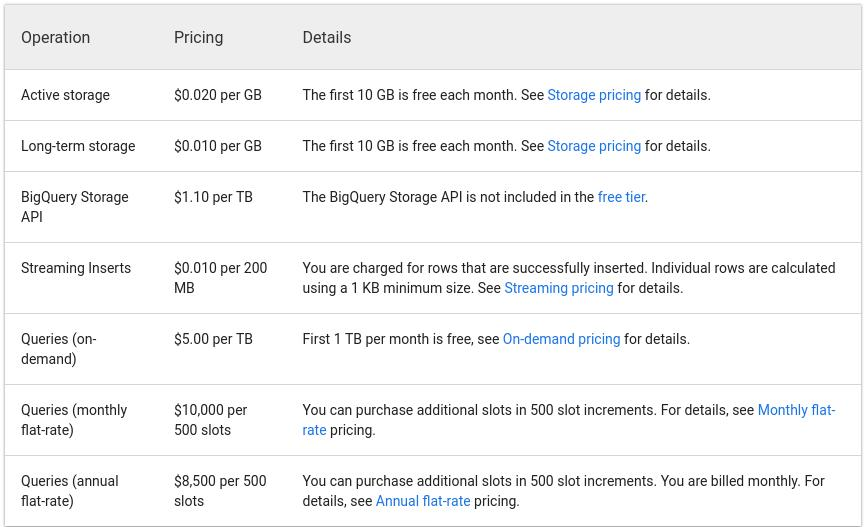
\includegraphics[width=0.7\linewidth]{BigQuerycosts}
	\end{figure}
	
\end{frame}

\begin{frame}{Data Store}
  - Part of Google Clouds DataStore
  -exists to save object oriented Datasets and Entities in NoSQL
  
  \begin{itemize}
  	\item[--] writes fast 
  	\item[--] provides SQL-like queries
  	\item[--] indexes
  	\item[--] ACID (atomicity, consistency, isolation, durability) $\rightarrow$ Data safety guaranteed
  	\item[--] mobile development 
  	\item[--] user profiles 
  	\item[--] product catalogues and inventory list and simple things like that
  	\item[--] Groups of Objects, Objects, Properties,  Unique ID as Key
  	
  \end{itemize}  
\end{frame}
\begin{frame}{Data Store}
	\centering
	\begin{figure}
		\centering
		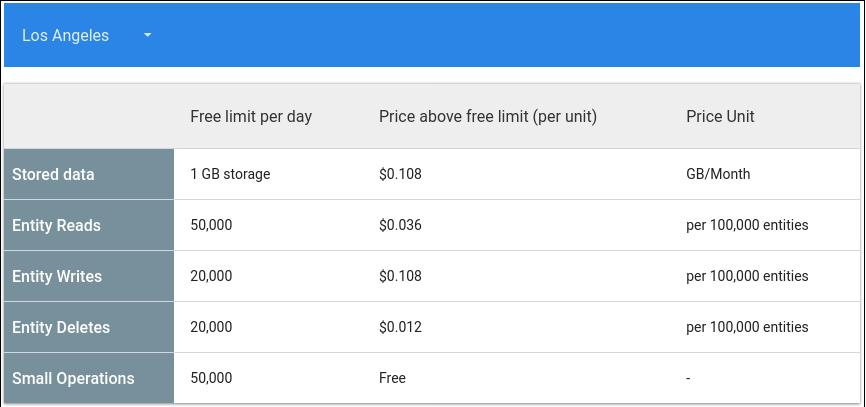
\includegraphics[width=0.7\linewidth]{datastorecosts}
	
		\label{fig: The Costs }
	\end{figure}
	
\end{frame}
\begin{frame}{Cloud storage}
	\begin{block}{}
     for files and pictures, works like any file manager, can be accessed via conventional code
	\end{block}
	\begin{outline}
		\1[--] standard for frequent access rate 
		
		\2[--] 2 ct up to  3.6 ct per GB 
		\1[--] nearline  
			
		\2 1 up to 2 ct per GB 
		\1[--] coldline
			
	\2	0.4 ct up to  0.9 ct per GB 
		
	\end{outline}

\end{frame}
\begin{frame}{App Engine Console}
	
	\$ gcloud app <command>\\
	
	\begin{enumerate}
		
		\item[--] browse 
		\item[--] create
		\item[--] deploy
		\item[--] describe 
		\item[--] open-console
	\end{enumerate}
\end{frame}
\begin{frame}{Memcache}
	\begin{block}{}
	But what does it do? 
	\end{block}
\end{frame}
\begin{frame}{Mem(e)cache}

\begin{block}

	But what does it do?
\end{block} \begin{center}

\includegraphics[width= 120pt, height=100pt]{potofgreed.jpg}
\end{center}

\begin{itemize}
\item literally a fucking  
	\colorbox{green!30}{memory cache}
\end{itemize}
\footnote{This page is just the conclusion of me messing with latex a bit and memeing. Of cause it won't be included in the final Form. Or will it be ?  }
\end{frame}

\begin{frame}{Memcache}
	
	\begin{center}
\textbf{	Shared Memcache:} \\
	\item it is shared between all users\\ \ \\
	
\textbf 	{Dedicated Memcache:}\\ 
	\begin{itemize}
		\centering
		\item Google offers up to 20 GB of memory cache for often used returns (100 on us-central!)
		\item as long as free it saves every request 
		\item 250 Byte key length (hashed if bigger) \\
		$\rightarrow$ more than enough 
		\item separate  set and get-hit
		\item 6 ct per GB/hour 
		\item writes at 5k items and reads 10k per  GB/s
	\end{itemize}

	\end{center}
\end{frame}


\begin{frame}{Restrictions}
	\begin{itemize}
		\item Apps can only use  Google intern filesystems (being the ones presented)
		\item only the aforementioned languages can be run, no c (or pyrex) modules for python code
		\item App Engine is only able to execute code called from an HTTP request\\
				\item \   
		\item \ 
		\item \ 
		\item \ 
				\item \ 
		\item \ 
		\item \ 
	
\end{itemize}
\end{frame}
\begin{frame}{Restrictions}
	\begin{itemize}
		\item Apps can only use  Google intern filesystems (being the ones presented)
		\item only the aforementioned languages can be run, no c (or pyrex) modules for python code
		\item App Engine is only able to execute code called from an HTTP request\\
	\colorbox{red}{BUT:}
		
		\begin{itemize}
			\item executed code can be called by itself via scheduled https requests as a workaround  
		\end{itemize}
	
		\item No sticky sessions.  
	\item No Maven for Java. 
		

	\end{itemize}
\end{frame}

\begin{frame}{Pro}
	\begin{itemize}
		\item Flexible pricing
		\item LOTS of potentially useful feature you don't have to integrate yourself
		\item No need to buy servers or server space (no maintenance)
		\item Makes solving the problem of scaling easier
		\item Free up to a certain level of consumed resources
		\item Suitable for apps that just store and retrieve data.
				\item $\rightarrow$  Nice option for start-ups/individuals $\leftarrow$ only need for a google account
		\item better peak performance than Amazon's EC2 service (more overall CPU hours)

	\end{itemize}
	
\end{frame}
\begin{frame}{Contra}
	\begin{itemize}
		\item No (easy) transferiability/migration. \\
		App Engine requires developers to use only its supported languages, APIs, and frameworks
		\begin{itemize}
		   \item There are open source project trying to fix this. 
		   \begin{itemize}
		   	\item Don't count on open source.
		   \end{itemize}
		\end{itemize}
	\item bulk downloads only for python (excluding java, php, go etc.)
	\item Not suitable for CPU intensive calculations. They are slower and expensive.	
	\end{itemize}
\end{frame}
\begin{frame}{Contra}
\begin{itemize}
	\item Suffers from traditional PaaS problems 
		\item relatively long development time for something rather simple, it has to be simple 
		\item if an app makes profit at Google scale then it probably  makes enough money to run on its own servers $\rightarrow$ scalability not worth
		\item lots of minor limitations making deep data analysis difficult
		\item sudden traffic spikes need a lot of inactive servers online $\rightarrow$ \$\$\$			for dealing with those		
	\end{itemize}
\end{frame}
\begin{frame}{Upper Limits of Using it for free  \footnote{https://www.icsr.agh.edu.pl/~malawski/google-appengine-ieee-2011.pdf}}
	\begin{itemize}
			\item Researchers used Taskline API to measure Google App Engine in great detail
		\item  Pipeline and Map API to build Framework to schedule and split task
		\item Used average computational steps / min to benchmark since amount of computational nodes is unknown/-predictable
		
	\end{itemize}

\end{frame}
	\begin{frame}{Upper Limits of Using it for free \footnote{https://www.icsr.agh.edu.pl/~malawski/google-appengine-ieee-2011.pdf}}
		\begin{figure}
			\centering
			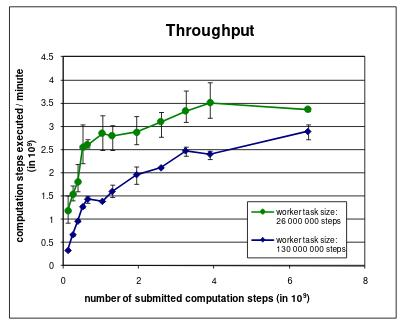
\includegraphics[width=0.7\linewidth]{Throughput}
		
			\label{fig:throughput}
		\end{figure}
	\end{frame}
\begin{frame}


	\begin{figure}
		\centering
		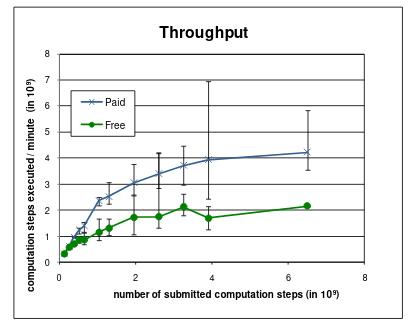
\includegraphics[width=0.7\linewidth]{Throughput2}
	
		\label{}
	\end{figure}
\end{frame}
\begin{frame}
	\begin{figure}
		\centering
		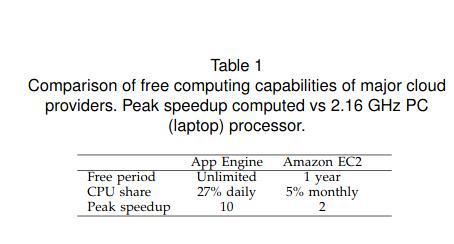
\includegraphics[width=0.7\linewidth]{Throughput3}
	
	
	\end{figure}
	
		
	\
	\end{frame}
\begin{frame}{Kudos}
	To..
	\begin{itemize}
		\item Wikipedia
		\item stack overflow
	\end{itemize}
\end{frame}

\end{document}
